% One harness, in the shape of the first sketch: a wrapper with snipped top corners around a
% document-shaped block of real C++. The wrapper holds the contract and its proof, the
% parameters, the empirical evidence and the runtime monitors.
% Build: pdflatex single-harness.tex    (the worked example is single-harness-detailed.tex)
\documentclass[border=8pt]{standalone}
\usepackage[T1]{fontenc}
\usepackage[default]{sourcesanspro}
\usepackage{tikz}
\usetikzlibrary{arrows.meta}
\definecolor{wrap}{HTML}{92C7E7}
\definecolor{edge}{HTML}{2F5B7C}
\definecolor{navy}{HTML}{14273A}
\begin{document}
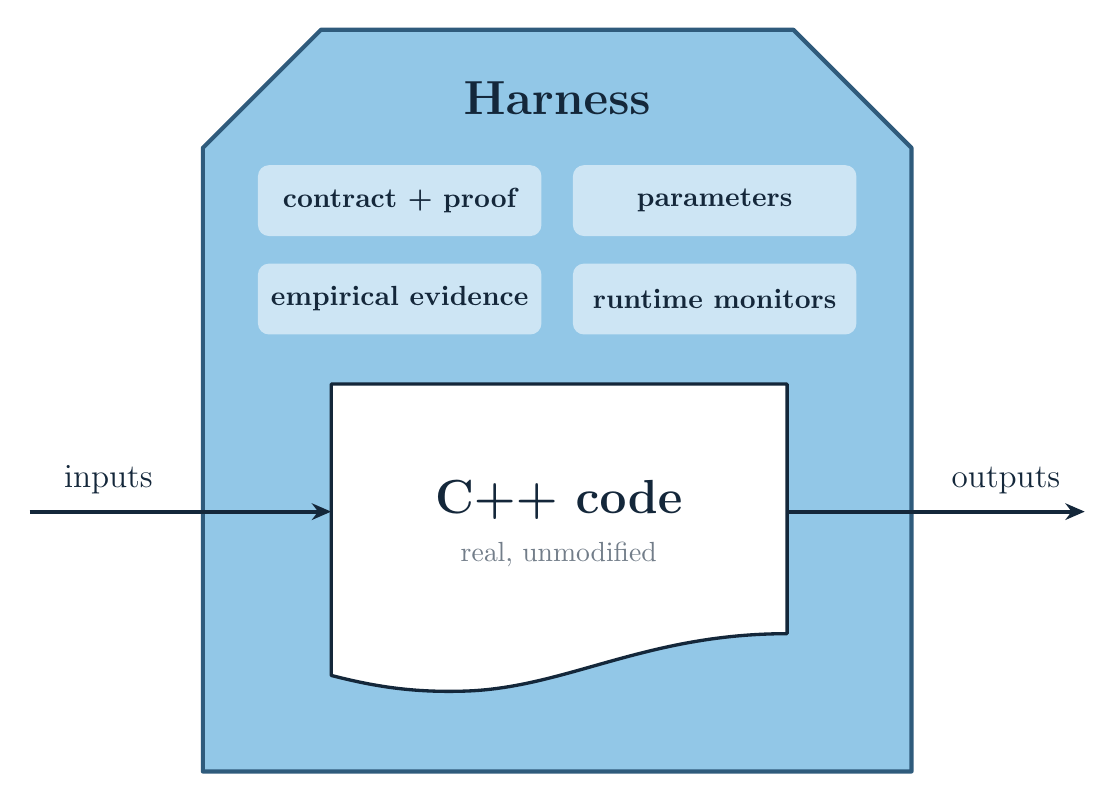
\begin{tikzpicture}[x=1cm,y=1cm,>={Stealth[length=7pt,width=6pt]},line join=round,
  item/.style={fill=white,fill opacity=0.55,text opacity=1,rounded corners=4pt,
               minimum width=3.6cm,minimum height=0.9cm,font=\bfseries,text=navy}]
% the wrapper
\draw[fill=wrap,draw=edge,line width=1.5pt]
  (0,0)--(9,0)--(9,7.92)--(7.5,9.42)--(1.5,9.42)--(0,7.92)--cycle;
\node[font=\bfseries\LARGE,text=navy] at (4.5,8.55) {Harness};

% what the wrapper holds
\node[item] at (2.5,7.25) {contract + proof};
\node[item] at (6.5,7.25) {parameters};
\node[item] at (2.5,6.0) {empirical evidence};
\node[item] at (6.5,6.0) {runtime monitors};

% the code block
\draw[fill=white,draw=navy,line width=1.2pt]
  (1.63,4.92)--(7.42,4.92)--(7.42,1.75)
  .. controls (5.6,1.75) and (4.6,1.05) .. (3.3,1.02)
  .. controls (2.6,1.0) and (2.1,1.1) .. (1.63,1.22)--cycle;
\node[font=\bfseries\LARGE,text=navy] at (4.52,3.45) {C++ code};
\node[font=\normalsize,text=navy!60] at (4.52,2.75) {real, unmodified};

% wires
\draw[line width=1.4pt,navy,->] (-2.2,3.3)--(1.63,3.3);
\draw[line width=1.4pt,navy,->] (7.42,3.3)--(11.2,3.3);
\node[anchor=south,font=\large,text=navy] at (-1.2,3.4) {inputs};
\node[anchor=south,font=\large,text=navy] at (10.2,3.4) {outputs};
\end{tikzpicture}
\end{document}
